\documentclass[11pt,a4paper]{report}
\usepackage[textwidth=37em,vmargin=30mm]{geometry}
\usepackage{calc,xunicode,amsmath,amssymb,paralist,enumitem,tabu,booktabs,datetime2,xeCJK,xeCJKfntef,listings}
\usepackage{tocloft,fancyhdr,tcolorbox,xcolor,graphicx,eso-pic,xltxtra,xelatexemoji}

\newcommand{\envyear}[0]{2025}
\newcommand{\envdatestr}[0]{2025-07-12}
\newcommand{\envfinaldir}[0]{webdb/2025/20250712/final}

\usepackage[hidelinks]{hyperref}
\hypersetup{
    colorlinks=false,
    pdfpagemode=FullScreen,
    pdftitle={Web Digest - \envdatestr}
}

\setlength{\cftbeforechapskip}{10pt}
\renewcommand{\cftchapfont}{\rmfamily\bfseries\large\raggedright}
\setlength{\cftbeforesecskip}{2pt}
\renewcommand{\cftsecfont}{\sffamily\small\raggedright}

\setdefaultleftmargin{2em}{2em}{1em}{1em}{1em}{1em}

\usepackage{xeCJK,xeCJKfntef}
\xeCJKsetup{PunctStyle=plain,RubberPunctSkip=false,CJKglue=\strut\hskip 0pt plus 0.1em minus 0.05em,CJKecglue=\strut\hskip 0.22em plus 0.2em}
\XeTeXlinebreaklocale "zh"
\XeTeXlinebreakskip = 0pt


\setmainfont{Brygada 1918}
\setromanfont{Brygada 1918}
\setsansfont{IBM Plex Sans}
\setmonofont{JetBrains Mono NL}
\setCJKmainfont{Noto Serif CJK SC}
\setCJKromanfont{Noto Serif CJK SC}
\setCJKsansfont{Noto Sans CJK SC}
\setCJKmonofont{Noto Sans CJK SC}

\setlength{\parindent}{0pt}
\setlength{\parskip}{8pt}
\linespread{1.15}

\lstset{
	basicstyle=\ttfamily\footnotesize,
	numbersep=5pt,
	backgroundcolor=\color{black!5},
	showspaces=false,
	showstringspaces=false,
	showtabs=false,
	tabsize=2,
	captionpos=b,
	breaklines=true,
	breakatwhitespace=true,
	breakautoindent=true,
	linewidth=\textwidth
}






\newcommand{\coverpic}[2]{
    % argv: itemurl, authorname
    Cover photo by #2~~(\href{#1}{#1})
}
\newcommand{\makeheader}[0]{
    \begin{titlepage}
        % \newgeometry{hmargin=15mm,tmargin=21mm,bmargin=12mm}
        \begin{center}
            
            \rmfamily\scshape
            \fontspec{BaskervilleF}
            \fontspec{Old Standard}
            \fontsize{59pt}{70pt}\selectfont
            WEB\hfill DIGEST
            
            \vfill
            % \vskip 30pt
            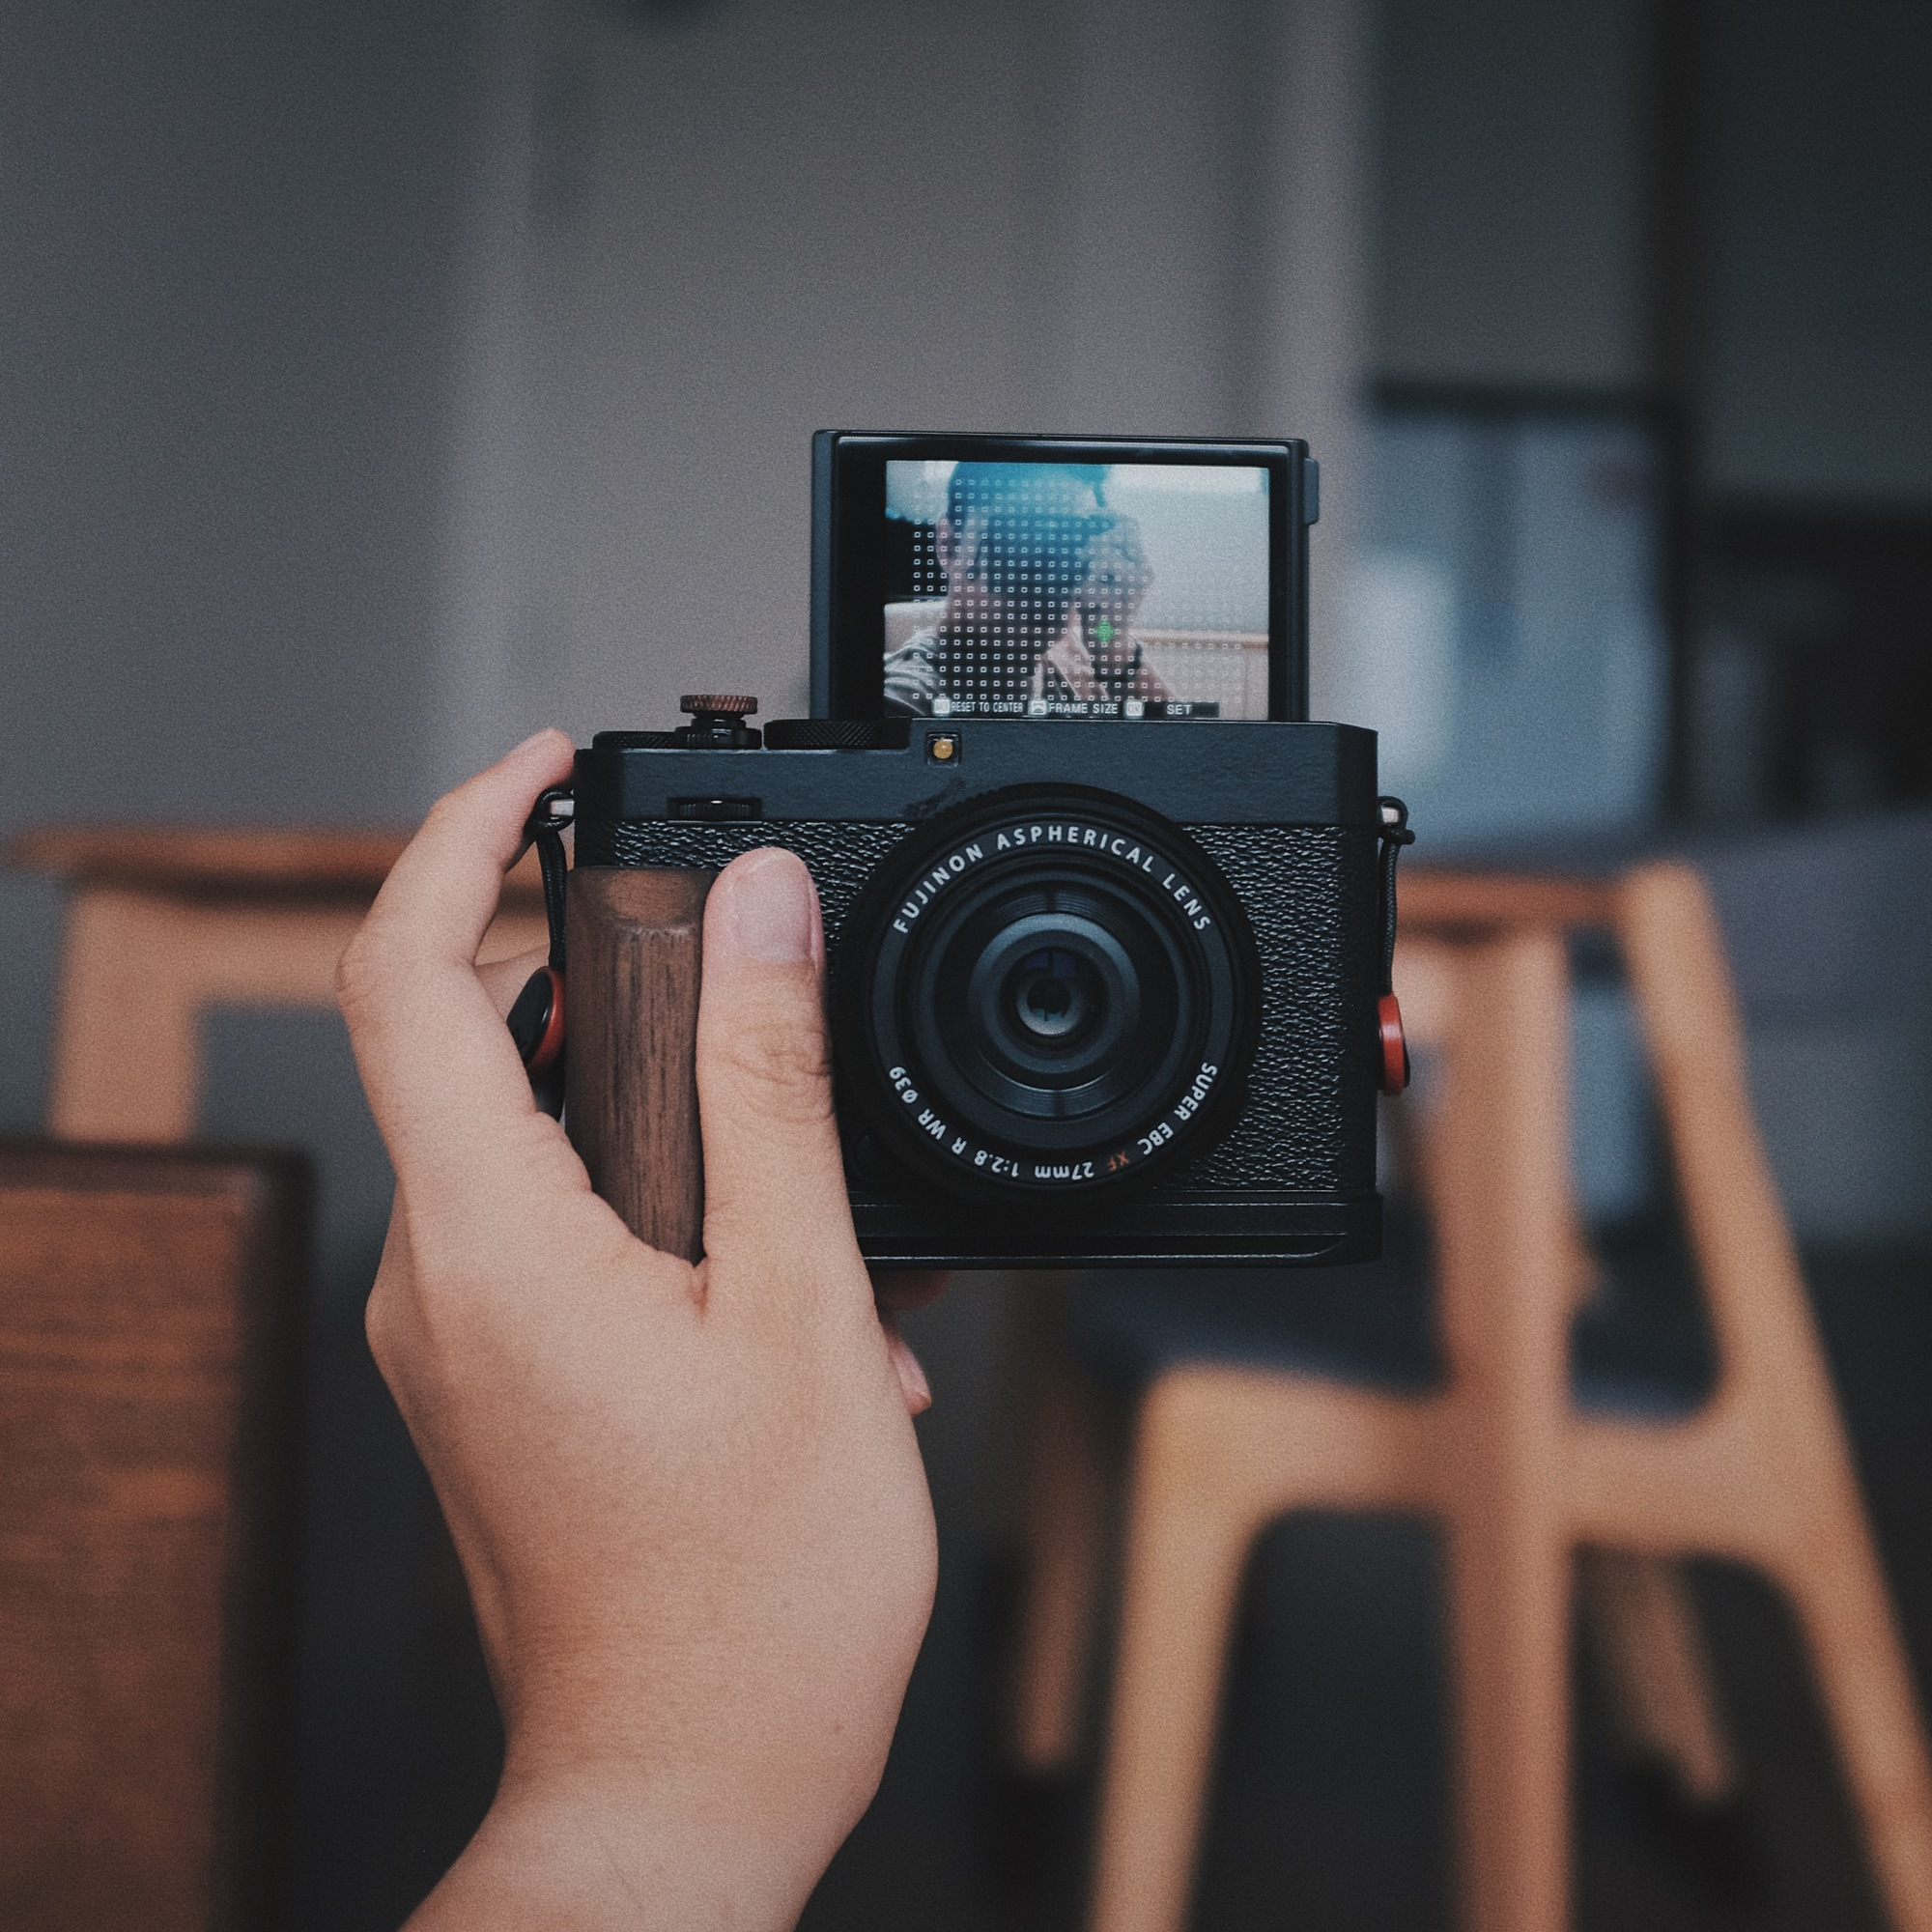
\includegraphics[width=\linewidth]{\envfinaldir/coverpic-prod.jpg}\par
            % \vskip 30pt
            \vfill

            \normalsize\rmfamily\scshape
            \copyright{} The Web Digest Project \hfill\large \envdatestr
        \end{center}
    \end{titlepage}
    % \restoregeometry
}
\newcommand{\simplehref}[1]{%
    \textcolor{blue!80!green}{\href{#1}{#1}}%
}
\renewcommand{\contentsname}{\center\Huge\sffamily\bfseries Contents\par\vskip 20pt}
\newcounter{ipartcounter}
\setcounter{ipartcounter}{0}
\newcommand{\ipart}[1]{
    % \vskip 20pt
    \clearpage
    \stepcounter{ipartcounter}
    \phantomsection
    \addcontentsline{toc}{chapter}{#1}
    % \begin{center}
    %     \Huge
    %     \sffamily\bfseries
    %     #1
    % \end{center}
    % \vskip 20pt plus 7pt
}
\newcounter{ichaptercounter}
\setcounter{ichaptercounter}{0}
\newcommand{\ichapter}[1]{
    % \vskip 20pt
    \clearpage
    \stepcounter{ichaptercounter}
    \phantomsection
    \addcontentsline{toc}{section}{\numberline{\arabic{ichaptercounter}}#1}
    \begin{center}
        \Huge
        \sffamily\bfseries
        #1
    \end{center}
    \vskip 20pt plus 7pt
}
\newcommand{\entrytitlefont}[1]{\subsection*{\raggedright\Large\sffamily\bfseries#1}}
\newcommand{\entryitemGeneric}[2]{
    % argv: title, url
    \parbox{\linewidth}{
        \entrytitlefont{#1}\par\vskip 5pt
        \footnotesize\ttfamily\mdseries
        \simplehref{#2}
    }\vskip 11pt plus 11pt minus 1pt
}
\newcommand{\entryitemGithub}[3]{
    % argv: title, url, desc
    \parbox{\linewidth}{
        \entrytitlefont{#1}\par\vskip 5pt
        \footnotesize\ttfamily\mdseries
        \simplehref{#2}\par\vskip 5pt
        \small\rmfamily\mdseries#3
    }\vskip 11pt plus 11pt minus 1pt
}
\newcommand{\entryitemAp}[3]{
    % argv: title, url, desc
    \parbox{\linewidth}{
        \entrytitlefont{#1}\par\vskip 5pt
        \footnotesize\ttfamily\mdseries
        \simplehref{#2}\par\vskip 5pt
        \small\rmfamily\mdseries#3
    }\vskip 11pt plus 11pt minus 1pt
}
\newcommand{\entryitemHackernews}[3]{
    % argv: title, hnurl, rawurl
    % \parbox{\linewidth}{
    %     \entrytitlefont{#1}\par\vskip 5pt
    %     \footnotesize\ttfamily\mdseries
    %     \simplehref{#3}\par
    %     \textcolor{black!50}{\href{#2}{#2}}
    % }\vskip 11pt plus 11pt minus 1pt
    \begin{minipage}{\linewidth}
            \entrytitlefont{#1}\par\vskip 5pt
            \footnotesize\ttfamily\mdseries
            \simplehref{#3}\par
            \textcolor{black!50}{\href{#2}{#2}}
    \end{minipage}\par\vskip 11pt plus 11pt minus 1pt
}







\begin{document}

\makeheader

\tableofcontents\clearpage




\ipart{Developers}
\ichapter{Hacker News}
\entryitemTwoLinks{OpenAI's Windsurf deal is off, and Windsurf's CEO is going to Google}{https://news.ycombinator.com/item?id=44536988}{https://www.theverge.com/openai/705999/google-windsurf-ceo-openai}

\entryitemTwoLinks{I'm more proud of these 128 kilobytes than anything I've built since}{https://news.ycombinator.com/item?id=44536248}{https://medium.com/@mikehall314/im-more-proud-of-these-128-kilobytes-than-anything-i-ve-built-since-53706cfbdc18}

\entryitemTwoLinks{ETH Zurich and EPFL to release a LLM developed on public infrastructure}{https://news.ycombinator.com/item?id=44535637}{https://ethz.ch/en/news-and-events/eth-news/news/2025/07/a-language-model-built-for-the-public-good.html}

\entryitemTwoLinks{jank is C++}{https://news.ycombinator.com/item?id=44534787}{https://jank-lang.org/blog/2025-07-11-jank-is-cpp/}

\entryitemTwoLinks{Pa. House passes 'click-to-cancel' subscription bills}{https://news.ycombinator.com/item?id=44533982}{https://www.pennlive.com/news/2025/07/pa-house-passes-click-to-cancel-subscription-bills-as-court-throws-out-federal-rule.html}

\entryitemTwoLinks{In a First, Solar Was Europe's Biggest Source of Power Last Month}{https://news.ycombinator.com/item?id=44533843}{https://e360.yale.edu/digest/solar-biggest-power-source-europe-june-2025}

\entryitemTwoLinks{Kimi K2}{https://news.ycombinator.com/item?id=44533403}{https://twitter.com/Kimi\_Moonshot/status/1943687594560332025}

\entryitemTwoLinks{Lead pigment in turmeric is the culprit in a global poisoning mystery (2024)}{https://news.ycombinator.com/item?id=44533337}{https://www.npr.org/sections/goats-and-soda/2024/09/23/nx-s1-5011028/detectives-mystery-lead-poisoning-new-york-bangladesh}

\entryitemTwoLinks{Top DNS domains seen on the Quad9 recursive resolver array each day}{https://news.ycombinator.com/item?id=44533055}{https://github.com/Quad9DNS/quad9-domains-top500}

\entryitemTwoLinks{Show HN: Vibe Kanban – Kanban board to manage your AI coding agents}{https://news.ycombinator.com/item?id=44533004}{https://github.com/BloopAI/vibe-kanban}

\entryitemTwoLinks{I'm done with social media – Or: why I have a blog now}{https://news.ycombinator.com/item?id=44532913}{https://www.carolinecrampton.com/im-done-with-social-media/}

\entryitemTwoLinks{Upgrading an M4 Pro Mac mini's storage for half the price}{https://news.ycombinator.com/item?id=44532306}{https://www.jeffgeerling.com/blog/2025/upgrading-m4-pro-mac-minis-storage-half-price}

\entryitemTwoLinks{Overtourism in Japan, and how it hurts small businesses}{https://news.ycombinator.com/item?id=44531707}{https://craigmod.com/ridgeline/210/}

\entryitemTwoLinks{AI agent benchmarks are broken}{https://news.ycombinator.com/item?id=44531697}{https://ddkang.substack.com/p/ai-agent-benchmarks-are-broken}

\entryitemTwoLinks{Things I learned from 5 years at Vercel}{https://news.ycombinator.com/item?id=44531635}{https://leerob.com/vercel}

\entryitemTwoLinks{Repaste Your MacBook}{https://news.ycombinator.com/item?id=44531569}{https://christianselig.com/2025/07/repaste-macbook/}

\entryitemTwoLinks{'Click-to-cancel' rule is blocked}{https://news.ycombinator.com/item?id=44531561}{https://apnews.com/article/ftc-click-to-cancel-30db2be07fdcb8aefd0d4835abdb116a}

\entryitemTwoLinks{At Least 13 People Died by Suicide Amid U.K. Post Office Scandal, Report Says}{https://news.ycombinator.com/item?id=44531120}{https://www.nytimes.com/2025/07/10/world/europe/uk-post-office-scandal-report.html}

\entryitemTwoLinks{Recovering from AI addiction}{https://news.ycombinator.com/item?id=44530922}{https://internetaddictsanonymous.org/internet-and-technology-addiction/signs-of-an-addiction-to-ai/}

\entryitemTwoLinks{Bill Atkinson's psychedelic user interface}{https://news.ycombinator.com/item?id=44530767}{https://patternproject.substack.com/p/from-the-mac-to-the-mystical-bill}


\ipart{Developers~~~~(zh-Hans)}
\ichapter{Solidot}
\entryitemGeneric{\hskip 0pt{}海洋中的纳米塑料多达数千万吨}{https://www.solidot.org/story?sid=81770}

\entryitemGeneric{\hskip 0pt{}GlobalFoundries 收购 MIPS}{https://www.solidot.org/story?sid=81769}

\entryitemGeneric{\hskip 0pt{}《星露谷物语》成为 Steam 平台最受好评的游戏}{https://www.solidot.org/story?sid=81768}

\entryitemGeneric{\hskip 0pt{}只有 1\% 的龟罹患癌症}{https://www.solidot.org/story?sid=81767}

\entryitemGeneric{\hskip 0pt{}Amarok 3.3 释出}{https://www.solidot.org/story?sid=81766}

\entryitemGeneric{\hskip 0pt{}基因组研究确认人类圈养动物后动物病毒开始传播给人类}{https://www.solidot.org/story?sid=81765}

\entryitemGeneric{\hskip 0pt{}西欧经历有记录以来最热的六月}{https://www.solidot.org/story?sid=81764}

\entryitemGeneric{\hskip 0pt{}两性权力关系泾渭并不分明}{https://www.solidot.org/story?sid=81763}

\entryitemGeneric{\hskip 0pt{}OpenAI 将发布 AI Web 浏览器挑战 Chrome  }{https://www.solidot.org/story?sid=81762}

\entryitemGeneric{\hskip 0pt{}麦当劳的 AI 招聘平台管理员密码是 123456}{https://www.solidot.org/story?sid=81761}

\entryitemGeneric{\hskip 0pt{}英伟达市值突破 4 万亿美元}{https://www.solidot.org/story?sid=81760}

\entryitemGeneric{\hskip 0pt{}美国科技巨头对财政部的制裁名单响应并不迅速}{https://www.solidot.org/story?sid=81759}

\entryitemGeneric{\hskip 0pt{}一群抹香鲸被拍摄到以站立姿态睡觉}{https://www.solidot.org/story?sid=81758}

\entryitemGeneric{\hskip 0pt{}230 万 Chrome 和 Edge 用户安装了会劫持浏览器会话的扩展}{https://www.solidot.org/story?sid=81757}

\entryitemGeneric{\hskip 0pt{}研究估计未来的胃癌病例大部分与幽门螺杆菌感染相关}{https://www.solidot.org/story?sid=81756}

\entryitemGeneric{\hskip 0pt{}海马体在成年后仍然能生成新神经元}{https://www.solidot.org/story?sid=81755}

\entryitemGeneric{\hskip 0pt{}海法洞穴发现的古代骨骼可能是人类和尼安德特人混血}{https://www.solidot.org/story?sid=81754}

\entryitemGeneric{\hskip 0pt{}科学家首次直接观测到反Klein隧穿现象}{https://www.solidot.org/story?sid=81753}\ichapter{V2EX}
\entryitemGeneric{\hskip 0pt{}[分享发现] Wispr Flow 推荐使用,多语种语音输入,很丝滑}{https://www.v2ex.com/t/1144686}

\entryitemGeneric{\hskip 0pt{}[问与答] 北京购买送白牌公牌的电动自行车能直接上路吗?}{https://www.v2ex.com/t/1144684}

\entryitemGeneric{\hskip 0pt{}[程序员] 前段时间领的免费 JetBrains 被取消了}{https://www.v2ex.com/t/1144683}

\entryitemGeneric{\hskip 0pt{}[问与答] 用 ChatGPT, Claude 的兄弟们都在国外吗?这两大陆香港都用不了}{https://www.v2ex.com/t/1144682}

\entryitemGeneric{\hskip 0pt{}[分享创造] SSL 证书申请工具 | 免费 HTTPS 证书网页在线申请 Let's Encrypt、ZeroSSL 等 HTTPS 证书 免登录}{https://www.v2ex.com/t/1144681}

\entryitemGeneric{\hskip 0pt{}[分享创造] Kiwi v1.1.0 发布了, 一款仿按键精灵的程序.}{https://www.v2ex.com/t/1144680}

\entryitemGeneric{\hskip 0pt{}[分享创造] PoPo: AI 生成 MMD 纸片人姿势}{https://www.v2ex.com/t/1144679}

\entryitemGeneric{\hskip 0pt{}[分享发现] [微信] 关闭其它人点赞/评论的提醒}{https://www.v2ex.com/t/1144678}

\entryitemGeneric{\hskip 0pt{}[职场话题] [校招生] 刚入职迷茫求助各位大佬}{https://www.v2ex.com/t/1144677}

\entryitemGeneric{\hskip 0pt{}[生活] 求助,怎么应对亲戚家孩子的无理行为?}{https://www.v2ex.com/t/1144675}

\entryitemGeneric{\hskip 0pt{}[Claude] claude code 还要排队?}{https://www.v2ex.com/t/1144674}

\entryitemGeneric{\hskip 0pt{}[Kubernetes] 请问大家所在公司的 k8s 集群 cni 和 cri 选型是什么?}{https://www.v2ex.com/t/1144673}

\entryitemGeneric{\hskip 0pt{}[问与答] 请教一下关于 Redhat 8.5 系统上 tls 握手失败的问题,非常感谢!}{https://www.v2ex.com/t/1144672}

\entryitemGeneric{\hskip 0pt{}[程序员] jb 真有格局!}{https://www.v2ex.com/t/1144669}

\entryitemGeneric{\hskip 0pt{}[问与答] 将一堆(七八块)闲置旧机械硬盘改造成家庭 NAS,有什么成熟方案?}{https://www.v2ex.com/t/1144667}

\entryitemGeneric{\hskip 0pt{}[SSL] 关于 Let's Encrypt 签发的证书 Ending OCSP Support in 2025 的后续问题}{https://www.v2ex.com/t/1144666}

\entryitemGeneric{\hskip 0pt{}[分享创造] 不懂前端,我花了 1 小时做了一个网页版游戏}{https://www.v2ex.com/t/1144665}

\entryitemGeneric{\hskip 0pt{}[程序员] 你现在的 ai 是?}{https://www.v2ex.com/t/1144664}

\entryitemGeneric{\hskip 0pt{}[问与答] 目前最强大的,支持克隆音色的语音合成模型是什么?}{https://www.v2ex.com/t/1144663}

\entryitemGeneric{\hskip 0pt{}[Chrome] chrome 上的 ublock 今天彻底寄了,有没有什么 chrome 的替代品,除了 edge}{https://www.v2ex.com/t/1144661}

\entryitemGeneric{\hskip 0pt{}[分享创造] 离谱,陌生人突然找到我,才发现是 3 个月前用 Cursor 做的自用番茄钟有流量了。。}{https://www.v2ex.com/t/1144660}

\entryitemGeneric{\hskip 0pt{}[前端开发] 请教一下前端问题}{https://www.v2ex.com/t/1144659}

\entryitemGeneric{\hskip 0pt{}[分享创造] 4 个月开发的 IOS 网球 AI 应用:小球圈}{https://www.v2ex.com/t/1144658}

\entryitemGeneric{\hskip 0pt{}[Apple] 关于 Live Photo,想请教各位前辈一个问题}{https://www.v2ex.com/t/1144657}

\entryitemGeneric{\hskip 0pt{}[JetBrains] 拍大腿系列:JetBrains 一年兑换码确认不回收}{https://www.v2ex.com/t/1144655}

\entryitemGeneric{\hskip 0pt{}[远程工作] 远程岗位: AI 模版开发招聘, ComfyUI ⼯作流开发⼯程师(Workflow Engineer)}{https://www.v2ex.com/t/1144653}

\entryitemGeneric{\hskip 0pt{}[酷工作] foya 传媒招聘到岗 PHP 30-50K}{https://www.v2ex.com/t/1144652}

\entryitemGeneric{\hskip 0pt{}[推广] 女娲:智能体平台}{https://www.v2ex.com/t/1144651}

\entryitemGeneric{\hskip 0pt{}[程序员] 做一个算命系统多少合适}{https://www.v2ex.com/t/1144650}

\entryitemGeneric{\hskip 0pt{}[分享创造] 周五晚上写了一个 mcp-echarts,来试试看!}{https://www.v2ex.com/t/1144649}

\entryitemGeneric{\hskip 0pt{}[Apple] 感觉现在注册新 apple 新账号风控比较严啊}{https://www.v2ex.com/t/1144648}

\entryitemGeneric{\hskip 0pt{}[酷工作] AI 产品经理(ComfyUI ⼯作流⽅向)}{https://www.v2ex.com/t/1144647}

\entryitemGeneric{\hskip 0pt{}[程序员] 历经一周总算完成了 Logo Hunter 的新版迭代}{https://www.v2ex.com/t/1144645}

\entryitemGeneric{\hskip 0pt{}[问与答] 求推荐一个月 20 元以内且流量超过 300G 的方案}{https://www.v2ex.com/t/1144644}

\entryitemGeneric{\hskip 0pt{}[程序员] 想搞台笔记本装 Linux 系统 求推荐!}{https://www.v2ex.com/t/1144643}

\entryitemGeneric{\hskip 0pt{}[问与答] [创业]看到有好几个小伙伴在分享创业的事, 我也分享下几个自己的小经验教训}{https://www.v2ex.com/t/1144642}

\entryitemGeneric{\hskip 0pt{}[生活] 有没有平时没事跑顺风车/滴滴的朋友?}{https://www.v2ex.com/t/1144641}

\entryitemGeneric{\hskip 0pt{}[问与答] 大家为什么对 manus 恶意这么大}{https://www.v2ex.com/t/1144640}

\entryitemGeneric{\hskip 0pt{}[酷工作] FOYA 传媒,招募火热进行中!欢迎各位技术大咖加入!}{https://www.v2ex.com/t/1144639}

\entryitemGeneric{\hskip 0pt{}[Claude] 没有买 Cursor 的用户还是用 Claude Code 吧}{https://www.v2ex.com/t/1144638}

\entryitemGeneric{\hskip 0pt{}[职场话题] 有家普通民企的 offer 但月工资里 50\% 是绩效,国内常态吗?大厂也是?}{https://www.v2ex.com/t/1144637}

\entryitemGeneric{\hskip 0pt{}[远程工作] 有网络工程师?可远程,可兼职}{https://www.v2ex.com/t/1144636}

\entryitemGeneric{\hskip 0pt{}[Vim] 求问 VS Code 中使用 Vim 插件, Normal 模式下 Tab 被接管了(Insert 模式下可以),没办法接受 AI 的代码提示,有无解决方法?}{https://www.v2ex.com/t/1144635}

\entryitemGeneric{\hskip 0pt{}[Chrome] Chrome 似乎已经彻底不支持旧版插件了}{https://www.v2ex.com/t/1144634}

\entryitemGeneric{\hskip 0pt{}[iOS] 急需 iOS 开发,有解决 4.3 上架 App Store 产品者优先}{https://www.v2ex.com/t/1144633}

\entryitemGeneric{\hskip 0pt{}[生活] 弟妹干脆决绝的离婚}{https://www.v2ex.com/t/1144632}

\entryitemGeneric{\hskip 0pt{}[程序员] 我的第一个 Directory 网站「极客盒子」终于上线了^\_^}{https://www.v2ex.com/t/1144631}

\entryitemGeneric{\hskip 0pt{}[生活] 运动手表高驰 pace pro 有什么可玩性吗}{https://www.v2ex.com/t/1144630}

\entryitemGeneric{\hskip 0pt{}[职场话题] 成都润芯微这家公司有人去过吗?怎么样?}{https://www.v2ex.com/t/1144628}

\entryitemGeneric{\hskip 0pt{}[奇思妙想] 一个必爆赚的非常有难度的科研项目}{https://www.v2ex.com/t/1144626}


\ipart{Generic News}







\clearpage
\leavevmode\vfill
\footnotesize

Copyright \copyright{} 2023-2025 Neruthes and other contributors.

This document is published with CC BY-NC-ND 4.0 license.

The entries listed in this newsletter may be copyrighted by their respective creators.

This newsletter is generated by the Web Digest project.

The newsletters are also delivered via Telegram channel \CJKunderline{\href{https://t.me/webdigestchannel}{https://t.me/webdigestchannel}}.\\
RSS feed is available at \CJKunderline{\href{https://webdigest.pages.dev/rss.xml}{https://webdigest.pages.dev/rss.xml}}.

This newsletter is available in PDF at
\CJKunderline{\href{https://webdigest.pages.dev/}{https://webdigest.pages.dev/}}.

The source code being used to generate this newsletter is available at\\
\CJKunderline{\href{https://github.com/neruthes/webdigest}{https://github.com/neruthes/webdigest}}.

This newsletter is also available in
\CJKunderline{\href{http://webdigest.pages.dev/readhtml/\envyear/WebDigest-20250712.html}{HTML}} and
\CJKunderline{\href{https://github.com/neruthes/webdigest/blob/master/markdown/\envyear/WebDigest-20250712.md}{Markdown}}.


\coverpic{https://unsplash.com/photos/a-stylish-graduate-poses-in-a-classroom-wzGkjFPA7ZY}{Christian Agbede}


\end{document}
